\documentclass{scrartcl}
\usepackage[margin=1in,a4paper]{geometry}
\usepackage[utf8]{inputenc}
\usepackage{amsfonts}         % for natural N
\usepackage{amsmath}          % for \text{}
\usepackage{indentfirst}      % to indent first line of section
\usepackage{hyperref}         % for \nameref{}
\usepackage{titlesec}         % for text next to section
\usepackage{mathabx}
\usepackage{tikz-qtree}

\renewcommand{\thesubsection}{}
\setlength{\parskip}{0.5em}   % spacing between paragraphs
\setlength\parindent{0pt}     % no indent at start of paragraphs

\titleformat{\section}[hang]
  {\normalfont\Large\bfseries}{\thesection}{1em}{}
\titleformat{\subsection}[runin]
  {\normalfont\large\bfseries}{\thesubsection}{1em}{}
  \titleformat{\subsubsection}[runin]
  {\normalfont\large\bfseries}{\thesubsubsection}{1em}{}

\title{Exercise 5}
\subtitle{Zero-Knowledge Proofs}
\author{Loïc Baccigalupi}

\begin{document}

\maketitle

\section*{5.2 The Permuted Kernel Problem}

\subsection*{i)}

For the protocol to be perfect complete, we need the $\text{Verify}$ calls to be always equal to $1$.
This implies that $Q\ ||\ HQ^{-1}\mathbf{w}$ and $R\ ||\ \mathbf{w} -bR\mathbf{v}$ need to be the correct messages for the commitments and openings $(A, d_A)$ and $(B, d_B)$ respectively, i.e.:

\begin{align*}
  \text{Commit}(pp, Q\ ||\ HQ^{-1}\mathbf{w}) &= (A, d_A) \\
  \text{Commit}(pp, R\ ||\ \mathbf{w} -bR\mathbf{v}) &= (B, d_B)
\end{align*}

Because $(A, d_A)$ and $(B, d_B)$ are computed at the start of the protocol, the two messages need to be computable from the start. We set $m_A = Q\ ||\ HQ^{-1}\mathbf{w}$ and $m_B = R\ ||\ \mathbf{w} -bR\mathbf{v}$.

We can fill in the first part as follows:
\begin{itemize}
  \item Generate $X \in \mathbb{Z}_2^{N \times N}$ and $\mathbf{r} \in \mathbb{Z}_2^N$ uniformly at random.
  \item Set $m_A = X\ ||\ HX^{-1}\mathbf{rv}$ and $m_B = XHP\ ||\ \mathbf{rv}$.
  \item Set $Q = X$ and $R = XHP$.
  \item Generate $\text{Commit}(pp, m_A) = (A, d_A)$ and $\text{Commit}(pp, m_B) = (B, d_B)$.
  \item Peggy has now computed $A$ and $B$.
\end{itemize}

In the second part, we set $\mathbf{w} = \mathbf{rv}$.

We now have:
\begin{align*}
  Q\ ||\ HQ^{-1}\mathbf{w} = X\ ||\ HX^{-1}\mathbf{rv} &= m_A \\
  R\ ||\ \mathbf{w} -bR\mathbf{v} = XHP\ ||\ \mathbf{rv} -bXHPv = XHP\ ||\ \mathbf{rv} &= m_B
\end{align*}
Which proves perfect correctness.

The protocol is also (2,2)-special-sound. The tree of accepting transcript is:

%\begin{tikzpicture}
%\Tree
%[.{$A, B$}
%      \edge node[auto=right] {a};
%      [.{$w_1$} {$Q_1, d_A$} {$R_1, d_B$} !{\qbalance} ]
%      [.{$w_2$} {$Q_2, d_A$} {$R_2, d_B$} !{\qbalance} ] ]

%\end{tikzpicture}
\begin{center}
  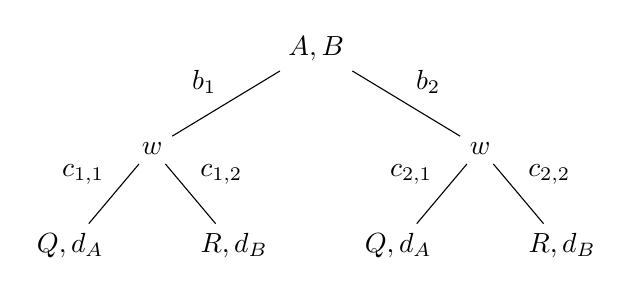
\begin{tikzpicture}[
    level distance=1.25cm,sibling distance=1cm,
    edge from parent path={(\tikzparentnode) -- (\tikzchildnode)}]
  \Tree
  [.{$A, B$}
     \edge node[auto=right] {$b_1$};
     [.{$w$}
        \edge node[auto=right] {$c_{1,1}$};
        [.{$Q, d_A$} ]
        \edge node[auto=left] {$c_{1,2}$};
        [.{$R, d_B$} ]
         ]
     \edge node[auto=left] {$b_2$};
     [.{$w$}
        \edge node[auto=right] {$c_{2,1}$};
        [.{$Q, d_A$} ]
        \edge node[auto=left] {$c_{2,2}$};
        [.{$R, d_B$} ]
         ]
  ]
  \end{tikzpicture}
\end{center}

Because at each branch, $c_{i,1} \neq c_{i, 2}$, the know that one leaf should have $Q, d_A$ and the other one $R, d_B$ (in the diagram, $c_{i,1} = 0$ and $c_{i, 2} = 1$ without loss of generality). \\
The extractor $E$ has then access to $Q$ and $R$ and can compute:

\begin{equation*}
  H^{-1}Q^{-1}R = H^{-1}X^{-1}XHP = H^{-1}HP = P
\end{equation*}

And succesfully extract the witness.


\subsection*{ii)} Proof of special honest-verifier zero-knowledge:

\subsubsection*{1) What is the verifier's view ?}\ \\
The verifier's view is: $(A, B, c, S, d_S)$, where $S \in \{A, B\}$ and $d_S \in \{d_A, d_B\}$.

\subsubsection*{2) What does the simulator do ?}
\begin{itemize}
  \renewcommand\labelitemi{--}
  \renewcommand\labelitemii{$\bullet$}
  \item If $c=0$:
  \begin{itemize}
    \item Generate $Q \in \mathbb{Z}_2^{N \times N}$ and $\mathbf{r} \in \mathbb{F}_2^N$ uniformly at random.
    \item Set $\mathbf{w} = \mathbf{rv}$.
    \item Compute $(A, d_A) = \text{Commit}(pp, Q\ ||\ HQ^{-1}\mathbf{rv})$.
    \item Generate $B \in \mathcal{C}$ uniformly at random. 
  \end{itemize}

  \item If $c=1$:
  \begin{itemize}
    \item Generate $R \in \mathbb{Z}_2^{N \times N}$ and $\mathbf{r} \in \mathbb{F}_2^N$ uniformly at random.
    \item Set $\mathbf{w} = \mathbf{rv}$.
    \item Compute $(B, d_B) = \text{Commit}(pp, R\ ||\ \mathbf{rv})$.
    \item Generate $A \in \mathcal{C}$ uniformly at random. 
  \end{itemize}
\end{itemize}

\subsection*{iii)}

\end{document}
